\documentclass[crop, tikz, border=.1cm]{standalone}
\usetikzlibrary{positioning}
\usetikzlibrary{calc}
\begin{document}
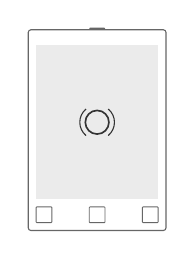
\begin{tikzpicture}
    \colorlet{border}{black!60}
\colorlet{screen}{black!8}
\colorlet{annotation}{black!80}

\newcommand\width{1.75}
\newcommand\height{2.55}
\newcommand\outborder{.1}
\newcommand\button{2 * \outborder}

\newcommand\definehighlightoption[3]{
    \ifcsname Highlight#1\endcsname
        \expandafter\newcommand\csname #1FillColor\endcsname{annotation}
        \expandafter\newcommand\csname #1DrawColor\endcsname{annotation}
    \else
        \expandafter\newcommand\csname #1FillColor\endcsname{#2}
        \expandafter\newcommand\csname #1DrawColor\endcsname{#3}
    \fi
}

\definehighlightoption{UpperKey}{border}{}
\definehighlightoption{HomeKey}{white}{border}

\tikzset{
    secondary/.style={line width=.3},
    back slate/.style={
        border, fill=white,
        rounded corners=1,
    },
    lower key/.style={
        draw=border, secondary, rectangle,
        rounded corners=0.25,
        minimum width={2 * \outborder cm},
        minimum height={2 * \outborder cm},
        inner sep=0pt,
    },
    upper key/.style={
        fill=\UpperKeyFillColor, rectangle,
        rounded corners=0.25,
        minimum width={2 * \outborder cm},
        minimum height=2pt,
        yshift=-.25pt,
        inner sep=0pt,
    },
}

\begin{scope}
    \node[upper key] at (.5 * \width, \height) (key-t) {};
    \draw[back slate] (0, 0) rectangle (\width, \height);

    \fill[screen]
        (\outborder, 4 * \outborder)
        coordinate (screen-bl)
        rectangle (\width - \outborder, \height - 2 * \outborder)
        coordinate (screen-tr);

    \coordinate (screen-c) at ($(screen-bl)!.5!(screen-tr)$);

    \node[lower key] at (2 * \outborder, 2 * \outborder) (key-l) {};
    \node[
        lower key,
        fill=\HomeKeyFillColor,
        draw=\HomeKeyDrawColor
    ] at (.5 * \width, 2 * \outborder) (key-c) {};
    \node[lower key] at (\width - 2 * \outborder, 2 * \outborder) (key-r) {};
\end{scope}

    \newcommand\innerradius{.15}
    \newcommand\outerradius{.22}
    \newcommand\partialangle{50}

    \draw[annotation, semithick] (screen-c) circle (\innerradius);

    \draw[annotation] ($(screen-c)+(\outerradius, 0)$)
         arc[radius=\outerradius, start angle=0, delta angle=\partialangle]
         ($(screen-c)+(\outerradius, 0)$)
         arc[radius=\outerradius, start angle=0, delta angle=-\partialangle];

    \draw[annotation] ($(screen-c)-(\outerradius, 0)$)
         arc[radius=\outerradius, start angle=180, delta angle=\partialangle]
         ($(screen-c)-(\outerradius, 0)$)
         arc[radius=\outerradius, start angle=180, delta angle=-\partialangle];
\end{tikzpicture}
\end{document}
